
\documentclass{article}
\usepackage{ijcai11}
\usepackage[dutch]{babel}
\usepackage{times}
\usepackage{gensymb}
\usepackage{graphicx}
\usepackage{float}
\usepackage{cite}
\usepackage{named}
\usepackage{url}
\usepackage{csquotes}
\hyphenpenalty = 10000
\exhyphenpenalty = 10000


\title{SmartLED-displays}
\author{Barbara Ameloot\\
KU Leuven\\
barbara.ameloot@student.kuleuven.be
\And 
Wouter Jochems\\
KU Leuven\\
wouter.jochems@student.kuleuven.be}

\pagenumbering{arabic}

\begin{document}
\fontsize{11pt}{13pt}\selectfont
\maketitle

\begin{abstract}
Deze paper onderzoekt een mogelijke toepassing van SmartLEDs, LEDs aangestuurd door een microcontroller\cite{smartLED}. Specifiek bestuderen we hun mogelijkheden op het gebied van LED-displays. LED-displays kennen veel toepassingen in verschillende gebieden, zoals marketing en entertainment. De fundamentele opbouw is vaak die van een centrale aansturing die het hele display bestuurt. Deze opbouw legt echter enkele beperkingen op en kan voor bepaalde problemen zorgen. We onderzoeken of een LED-display opgebouwd uit SmartLEDs, waarbij er geen centrale aansturing is, een meerwaarde biedt ten opzichte van de beperkingen die we bij de klassieke displays vaststellen. We concluderen dat SmartLED-displays niet altijd een goede vervanging zijn voor conventionele LED-displays, maar wel extra mogelijkheden bieden voor meer experimentele LED-displays.
\end{abstract}

{\bf Keywords:} SmartLED, VLC, LED, LED Display, Arduino, Microcontroller,


\section{Introductie}

LED-displays worden vaak gebruikt op evenementen en reclameborden. De huidige displays werken meestal met een centrale aansturing. Deze opbouw zorgt echter voor beperkingen bij het gebruik van de displays. Wij identificeren drie beperkingen waarvoor we onderzoeken of een SmartLED-display, zonder centrale aansturing, een meerwaarde kan bieden.

\begin{figure}
\centering
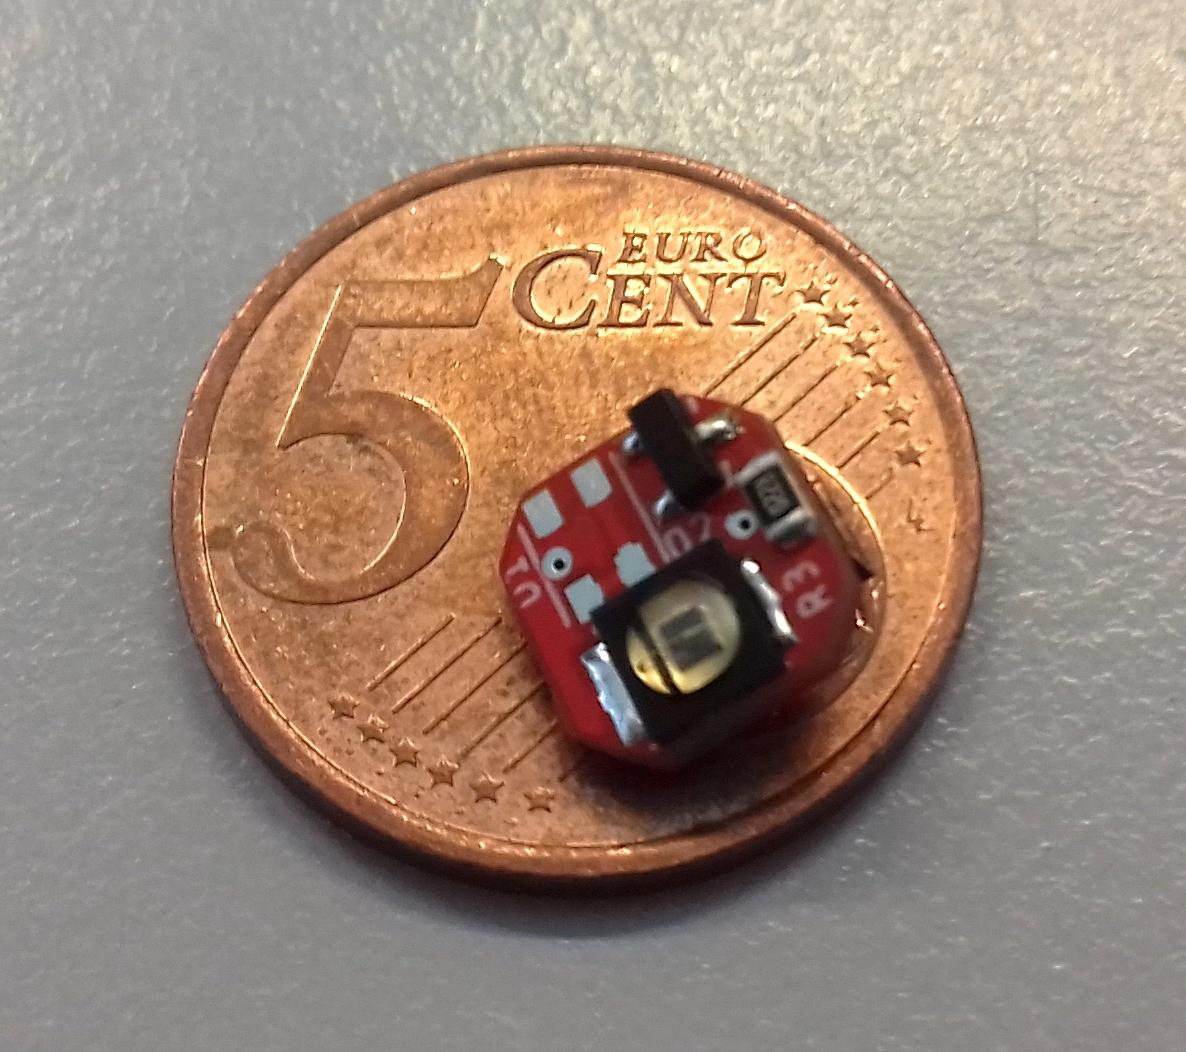
\includegraphics[width=6cm]{SmartLED.png}
\caption{Een SmartLED}
\end{figure}

\begin{enumerate}


\item Een eerste punt is flexibiliteit. Er zijn reeds flexibele displays beschikbaar. Omdat elke led vanuit een centraal punt wordt aangestuurd is het nodig dat deze centrale controller kennis heeft van de positie van de LEDs. Dit zorgt ervoor dat de huidige flexibele displays beperkt zijn in hun bewegingsmogelijkheden. De individuele LEDs zijn vaak aangesloten op een raster of slinger om de relatieve positie van de LEDs ten opzichte van elkaar te behouden. Door de centrale controller weg te laten denken wij de nood aan het behouden van de relatieve posities te elimineren. Dit leidt tot meer mogelijkheden voor de dynamische flexibiliteit van een SmartLED-display.

\item Een tweede punt is interactiviteit. Ook hier zijn er reeds interactieve displays op de markt. Deze zijn echter vaak rigide. Door elke SmartLED van een eigen micro-controller te voorzien zorgen we ervoor dat deze zelf signalen van buitenaf kan verwerken. De individuele LEDs zijn bijgevolg onafhankelijk van andere besturingselementen toch in staat om in interactie te treden met de buitenwereld. Voor deze interactie maken we gebruikt van een “lichtpen”, dit is een SmartLED die een gebruiker op het display kan richten om zo signalen over te brengen aan de hand van infrarood licht.

\item Als derde en laatste punt bekijken we modulariteit. Zoals eerder vermeld zijn is de flexibiliteit van de huidige displays beperkt. Doordat de LEDs vanuit één centraal punt worden aangestuurd zullen problemen bij de centrale controller een impact hebben op het hele display. Ook is het vaak moeilijk om een individuele LED of groepen van LEDs te vervangen wanneer deze niet meer werken. Door elke SmartLED als individuele entiteit te laten functioneren kunnen problemen zich niet voortplanten over het display. Omdat de SmartLEDs enkel afhankelijk zijn van zichzelf is het ook makkelijk om een enkele led te vervangen.
\end{enumerate}

\begin{figure}[H]
\centering
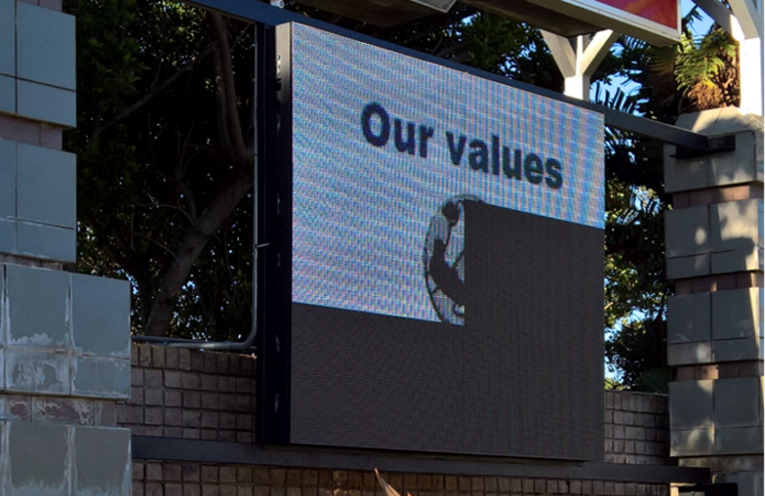
\includegraphics[width=8cm]{broken.png}
\caption{Een LED-display met verbindingsproblemen}
\end{figure}

\section{Verwant werk}
Dit project is een rechtstreeks vervolg op het project van vorig jaar waarin de SmartLEDs ontwikkeld werden. \cite{smartLED}
Daarnaast is er al veel onderzoek gebeurd rond LEDs en hun mogelijk tot signaaloverdracht. Zo werd er al door ETH Zurich en Disney research onderzoek gedaan naar de mogelijkheden van VLC, visual light communication, networks waarbij verschillende microcontrollers met elkaar communiceerden via LEDs \cite{VLCNetworks}.  Verder is er nog project firefly\cite{firefly} waarbij reeds een werkend display werd opgebouwd van individueel aangestuurde LEDs maar deze waren nog steeds verbonden via een kabel.



\section{Evaluatie}

Het doel van ons onderzoek is nagaan of een display opgebouwd uit SmartLEDs een meerwaarde biedt ten opzichte van gewone displays. Hiervoor bekijken we de drie beperkingen die we vaststellen bij de klassieke displays: flexibiliteit, interactiviteit en modulariteit. Daarnaast onderzoeken we welke bijkomende beperkingen een SmartLED-display heeft.

Met \textbf{flexibiliteit} bedoelen we dat het mogelijk moet zijn om de SmartLEDs te verplaatsen zonder dat hiervoor code moet worden aangepast. Dit betekent dat de communicatie met en door de SmartLEDs onafhankelijk moeten werken van hun positie in het display. 

Voor de \textbf{interactie} willen we dat deze op een betrouwbare en interactieve manier gebeurt. Hiervoor maken we gebruik van een "lichtpen". Dit is een SmartLED voorzien van enkele knoppen om zo input door te sturen naar het display. Aan de hand van een floodlight, een lichtpen voorzien van meerdere, krachtigere LEDs, kunnen grotere groepen SmartLEDs aangestuurd worden. Het moet dus mogelijk zijn om aan de hand van een SmartLED een signaal te geven aan een andere SmartLED.

Voor \textbf{modulariteit} is het belangrijk dat er SmartLEDs kunnen worden toegevoegd en weggelaten zonder dat dit een invloed heeft op de rest van het display. Dit hangt nauw samen met de flexibiliteit. Waar we bij flexibiliteit vooral kijken naar de verplaatsbaarheid van LEDs, leggen we hier de focus op het toevoegen en weglaten van SmartLEDs. Hier is het vooral belangrijk dat het niet uitmaakt welke LEDs er deel uitmaken van het display. 



\section{Opstelling}
De uiteindelijke implementatie zou gebruik maken van SmartLEDs. Om praktische redenen waren wij niet in staat deze te gebruiken tijdens ons onderzoek. 
Om onze hypothese te testen maken we gebruik van LEDs verbonden met Zigduino r2 microcontrollers. De Zigduino’s bevatten een infrarood led en een RGB led. We kiezen ervoor om een infrarood led toe te voegen omdat dit de communicatie een stuk minder complex maakt. Indien we gebruik zouden maken van zichtbaar licht, zoals bij VLC, is het nodig om rekening te houden met het omgevingslicht. Dit veranderd voortdurend en deze verandering moet in rekening gebracht worden om onderscheidt te maken van een doelbewust signaal en het aanwezige omgevingslicht. De veranderingen in het aanwezige infrarood licht zijn veel minder uitgesproken. Dit laat ons toe om de threshold, de waarde vanaf wanneer we een signaal registreren, redelijk constant te houden. Om deze reden stappen we af van de pure VLC en kiezen we ervoor een extra infrarood LED toe te voegen.


\section{Methode}

Voor het schrijven van de code\footnote{Alle code is beschikbaar op \\ https://github.com/WoodyJo/SmartLED-displays} gebruiken we de standaard Arduino IDE.


\subsection{Onderlinge communicatie}

Voor de communicatie tussen SmartLEDs zijn we vertrokken vanuit VLC, visual light communication. Zoals \cite{VLCNetworks} aantoont is het mogelijk om LEDs te gebruiken om zowel licht uit te zenden als te ontvangen. Dit kan gebruikt worden voor communicatie tussen LEDs onderling zonder dat dit merkbaar is voor een gebruiker; de LED lijkt altijd aan, zo blijkt uit de paper. De communicatie verloopt grotendeels zoals beschreven in \cite{smartLED}. Met als uitzondering de schakeling van de LED. 

\subsubsection{Reverse Bias}
We hebben gemerkt dat het verschil tussen de gemeten waarde wanneer we wel of niet op de LED schijnen veel groter is wanneer we de infrarood LED in \textbf{reverse bias} schakelden, in tegenstelling tot de forward bias zoals in \cite{smartLED} gebruikt wordt. Dit vermoeden wordt bevestigd door de resultaten in tabel 1. Deze geeft telkens de waarden weer die door de Zigduino over de LED worden gemeten. Zoals beschreven in de Arduino Referentie \cite{Arduino} bevat het bord een analog to digital converter. Deze mapt het input voltage op integer waarden tussen 0 en 1023. Bij de Zigduinos gebeurt dit op dezelfde manier. De tabel geeft een gemiddelde van 30 metingen van deze integer waarden zoals gemeten met de lichtbron op verschillende afstanden, alsook zonder de lichtbron. 

Om het verschil tussen de forward bias en reverse bias te bevestigen bekijken we de waarden voor een afstand van 8 cm. Dit lijkt ons een representatieve afstand voor de communicatie met de lichtpen. We bekijken het absolute verschil tussen de waardes met en de waardes zonder lichtbron. 
Voor de forward bias zien we een absoluut verschil van 27. Dit bedraagt slechts 6,96\% van de standaardwaarde zonder licht. 
Voor de reverse bias zien we een absoluut verschil van 712, ofwel 98,6\% van de standaardwaarde zonder licht. 
Door het grote verschil in waarde is het makkelijker om te registreren wanneer er effectief een signaal naar de LED wordt gestuurd in plaats van eventuele ruis. We plaatsen de infrarood LED dus in reverse bias.


\begin{table}
	\centering
    \begin{tabular}{ | p{1.5cm} | p{1.5 cm} | p{1.5 cm} | }
    \hline
    & & \\
    Afstand tot lichtbron (in cm) & Reverse Bias gemeten waarde & Forward Bias gemeten waarde  \\ \hline
    & &  \\
    4 & 0 & 425  \\ 
    6 & 3 & 418   \\ 
    8 & 10 & 416   \\ 
    10 & 24 & 413   \\ 
    15 & 330 & 405   \\ 
    20 & 380 & 397  \\ 
    30 & 515 & 388  \\ \hline
    & & \\ 
    Geen extra lichtbron & 722 & 388   \\ 

    \hline
    \end{tabular}
  \caption{Gemeten waarden over LED} 
\end{table}

\subsubsection{Synchronisatie}

 Voor de \textbf{synchronisatie} maken we gebruik van oversampling, zoals beschreven in de paper. Dit houdt in dat we voor elke bit meerdere lezingen uitvoeren, namelijk 3. Door de metingen met elkaar te vergelijken kunnen onverwachte veranderingen worden opgespoord. Hieruit kan worden afgeleid of de lezer voor of achterloopt op de zender. Om ervoor te zorgen dat de juiste bitstring gelezen wordt, zal de lezer de fout corrigeren door de laatste meting van de vorige bit over te brengen naar de volgende. Voor de volgende bit worden dan maar 2 bijkomende metingen gedaan.
 
\subsubsection{Threshold}

Om ervoor te zorgen dat de SmartLEDs een verschil zien tussen omgevingslicht en een signaal moeten we een threshold, een waarde vanaf wanneer we een meeting als input beschouwen, instellen. Omdat we gebruik maken van infraroodlicht blijft de waarde van de threshold redelijk constant. We merken echter wel verschillen in de gemeten basiswaarde afhankelijk van het gebruikte Zigduino-bord en eventuele storingsbronnen. Hierdoor is het nodig om op regelmatige tijdstippen de waarde van de threshold bij te sturen. 
Wanneer we de gemeten waarde zonder lichtinput plotten krijgen we een duidelijk sinusoïdale verloop zoals te zien op figuur 2. Dit valt te verklaren door de RC-kringen in de gebruikte zigduino’s die als oscillator werken. \cite{oscillator}  

\begin{figure}[H]
\centering
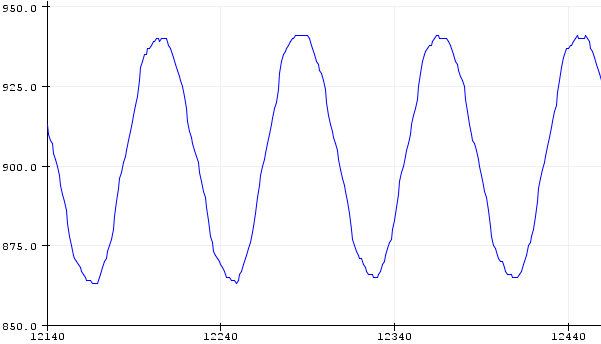
\includegraphics[width=8cm]{ruis.png}
\caption{De gedetecteerde ruis, gemeten spanning in functie van de tijd}
\label{fig:ruis}
\end{figure}

Om de gemeten waarde van het omgevingslicht nauwkeuriger te maken besloten we om deze gelijk te stellen aan het gemiddelde van tien metingen met telkens 50ms (ongeveer de helft van een periode) tussen om het sinusoïdale verloop op te vangen. Hierbij tellen we een waarde op, die groter is dan de amplitude van de sinus golf, en bekomen zo onze threshold. 
Voor ons onderzoek volstaat het om de threshold te bepalen wanneer de SmartLED wordt geactiveerd of een nieuw programma wordt uitgevoerd.

\subsection{Eigenschappen display}

Om de LEDs als één display te laten werken, zoeken we een manier om een signaal door te geven tussen de LEDs. Hiervoor wilden we aanvankelijk gebruik maken van de aanwezige infrarood LED. We zijn er echter niet in geslaagd om een zijdelings signaal door te geven indien de LEDs beiden naar boven wijzen. Dit is te verklaren door de beperkte stralingshoek van de LED, zoals geïllustreerd in figuur 3.

\begin{figure}[H]
\centering
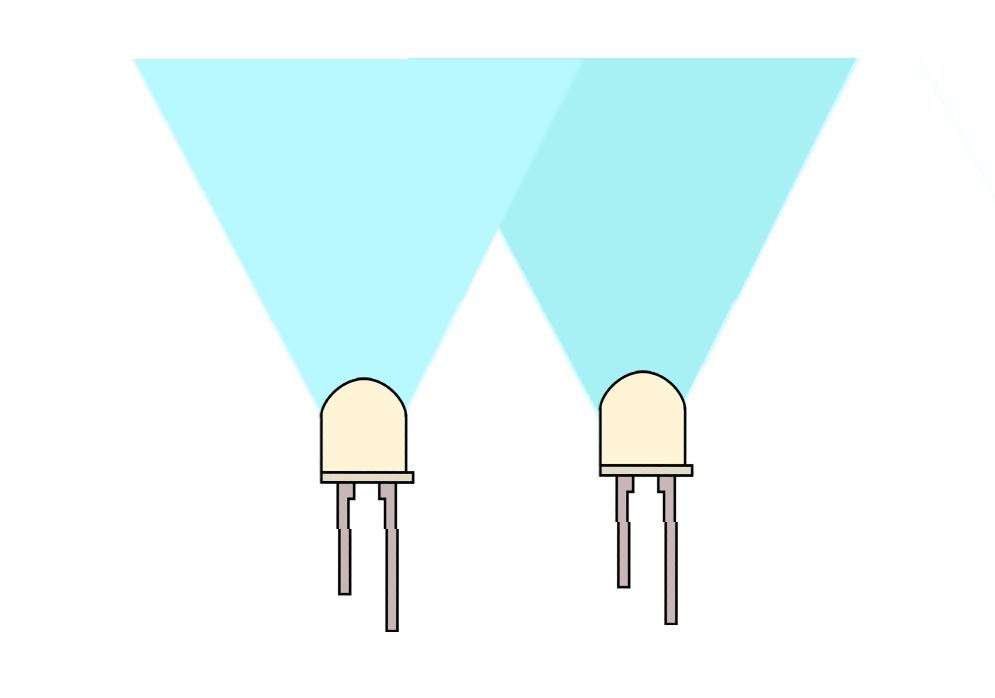
\includegraphics[width=8cm]{LedNaastElkaar.png}
\caption{Stralingshoek bij zijdelings gepositioneerde LEDs}
\label{fig:ruis}
\end{figure}

Een mogelijke oplossing hiervoor zou het gebruiken van een diffuser kunnen zijn om zo een grotere stralingshoek te bekomen. Wij hebben dit in onze opstelling getest aan de hand van een pingpong bal. Dit bleek in ons geval echter niet voldoende om de zijwaartse communicatie te doen slagen. Door een krachtigere LED te gebruiken, d.w.z. een die meer lumen produceert, zou dit mogelijk toch een oplossing kunnen zijn. Dit hebben wij niet verder onderzocht. 

Een andere mogelijkheid zou zijn om dit op te lossen door extra infrarood LEDs te monteren die naar de buitenkant gericht zijn, in plaats van naar boven. Wij hebben er echter voor gekozen dit niet te doen omdat we de smartLEDs zo eenvoudig mogelijk wilden houden. 

Deze keuze resulteert echter wel in een beperking voor eventuele toepassingen van het display:
\medskip
\begin{displayquote}

 \textit{Er is geen zijwaartse communicatie tussen de individuele smartLEDs.}
\end{displayquote}
\medskip


Met twee naar elkaar gerichte LEDs lukt het ons wel om een bit-string door te zenden. Deze opstelling bestaat uit een eerste LED die een bit-string uitzendt, een tweede die deze ontvangt en doorgeeft aan een microcontroller en vervolgens een derde die de ontvangen bit-string weer uitzendt in een andere richting. In minder conventionele LED-displays (met een vorm die het toelaat de LEDs naar een elkaar te richten of met bewegende onderdelen) is onderlinge communicatie dus wel mogelijk.

\subsection{Meerdere LEDs}
Bij aanvang van ons project hoopten we voor het display en het verzenden van informatie dezelfde LED te gebruiken. Dit is niet alleen compacter dan met meerdere LEDs maar het zorgt er ook voor dat we de SmartLED niet moeten uitbreiden met extra hardware. Helaas bracht dit extra moeilijkheden met zich mee, zoals informatie die verzonden moest worden over een LED die volgens het display geen licht mag uitzenden. Ook maakte dit onze code veel complexer.

Om deze redenen kozen we om met een tweede LED te werken. Ook besloten we om de communicatie via een infrarood LED te laten verlopen, zo vermijden we dat de communicatie-LEDs signalen zouden opvangen van de display-LEDs. Bovendien creëert dit meer mogelijkheden voor het display aangezien het volledige RGB spectrum kan gebruikt worden om afbeeldingen weer te geven. 

\subsection{Externe lichtbron}
Omdat een tweede LED ook een externe lichtbron is, valt uit het voorgaande al te besluiten dat een goed gericht licht in staat is om te interageren met een SmartLED-display. 

Wij onderzochten twee manieren waarop interactie met het LED-display mogelijk was. Dit aan de hand van een lichtpen (een LED met een microcontroller achter) die op een bepaalde manier geprogrammeerd was.

De eerste manier bestond uit een reactie van het display wanneer een signaal verzonden werd, versus wanneer er geen verzonden werd. We programmeerden hiervoor een soort "\textit{Whack-a-mole}" spel waarbij de speler een bepaalde tijd heeft om te reageren op een licht verandering door de lichtpen hierover te laten schijnen. Zowel bij succes als bij mislukking geeft het display feedback door weer van licht te veranderen (zie figuur \ref{fig:mole}).
\begin{figure}
\centering
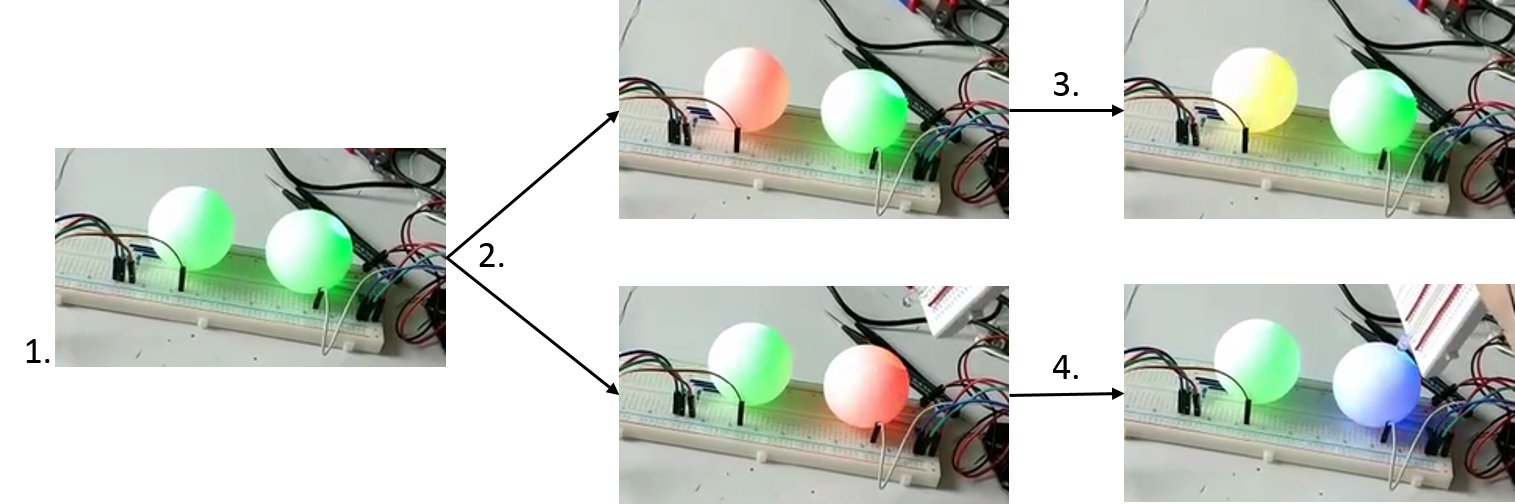
\includegraphics[width=8cm]{moleSequence.png}
\caption{1:inactief, 2:vraagt om respons, 3:geen respons, \mbox{4: wel respons}}
\label{fig:mole}
\end{figure}
Bij de tweede manier wordt er een bit-string verzonden naar het display. Deze manier hebben we getest met een programma waarbij een bit-string gelijk werd gesteld aan een kleur die de display LED moest aannemen of aan een programma dat afgespeeld moest worden.


\section{Conclusie}
Conventionele LED-displays komen vooral vlak voor en dit is helaas niet echt mogelijk met SmartLED-displays aangezien zo geen communicatie mogelijk is. Hieruit besluiten we dat SmartLED-displays geen alternatief zijn voor conventionele LED-displays. Ze bezitten echter wel bepaalde eigenschappen die ze niet alleen bruikbaar maar ook bijzonder maken. Ze kunnen interactief gebruikt worden als simpele, vlakke displays zonder onderlinge communicatie maar ook zonder eventuele verbindingsproblemen. Daarnaast kunnen ze in andere vormen wel signalen doorgeven en dus meer als 1 geheel functioneren.


\section{Verder werk}
Als vervolg op dit project zou een display opgebouwd uit echte SmartLEDs gemaakt kunnen worden. Het zou ook interessant zijn mocht er een oplossing gevonden worden voor het probleem met de invalshoek van de LEDs zodat zijdelings gecommuniceerd kan worden.

\bibliography{bronnen}
\bibliographystyle{named}

\end{document}

